%%%%%%%%%%%%%%%%%%%%%%%%%%%%%%%%%%%%%%%%%%%%
%%% OCCULTISM
%%%%%%%%%%%%%%%%%%%%%%%%%%%%%%%%%%%%%%%%%%%%

\newpage


\mysection{Occultism}{cunning-occultism}

\callout {
    \mytable{Y Y} {
        \thead{\# Pips} & \thead{Coin per Pip} \\
    } {
        1-5 & 100\FE \\
        6-10 & 100\AG \\
        11+ & 100\AU
    }
}


\myimage{cunning/CunningHound}

\OCCULT[
  Name=Barghest,
  Link=occultism-barghest,
  Pips=5,
  Time=Days
]

You summon a spectral black dog (a harbinger of death and misfortune) to torment a single person for 7 days.  You must whisper the birth name of the victim to the spectre; upon hearing it, the black dog will seek the victim out, traveling up to 100km a night to find them.  The barghest can only travel at night, and disappears at the first light of the rising sun.  The dog can see invisible or hidden creatures and will unerringly find the target provided they are within distance of the casting of the ritual.

Once found, the barghest will appear to the victim once every night.  The victim is permitted a \SAVE{Doom} when they see the Barghest; if they fail, they suffer the curse of the Barghest until it appears again at sunset.  Pooka are immune to Barghests, and if the victim is in a Band with the Pooka, they get two Saves.

If the victim fails their save, they suffer the following maledictions until the next sundown:

\callout {
\mybullet {
    \item They are unable to heal Grit.
    \item All \RO and \RB tests suffer a -4 penalty.
    \item All of their \mylink{Kismet}{adventurer-kismet} dice move \DCDOWN.
}}

The victim must be someone Hallowed and Mortal.  The ritual requires a dog (your familiar is fine) and an item belonging to the victim. No harm comes to the dog, but the spectral figure will resemble him or her if examined closely.

\OCCULT[
  Name=Bind Familiar,
  Link=occultism-bind-familiar,
  Pips=2,
  Time=Weeks
]

Your Familiar is an embodiment of the Void, bound to your soul.  They can be summoned and dismissed at will: they'll appear from a shadow (cat) or sewer grate (rat) or fly in through a window (raven), and they'll leave roughly the same way.  Familiars are Unhallowed, and grant you +1 Cunning Pip if they're with you when you practice Occultism.

Familiars can be sent on missions up to 10km away. By Concentrating, you can "link" your mind with theirs. In this state you can see what they see and hear what they hear.  While Concentrating, you can cast \mylink{Charms}{vulgate-charms} through your Familiar if you desire (should you know the Vulgate of Charms). While linked with your Familiar you can remember things your familiar remembers (so you could send them on a spying mission and later "remember" what they saw). While Familiars are themselves immune to \mylink{Secrets of the Mind}{arcana-wizardry-secrets-alignment}, if one of these Secrets is performed on them while you are linked you will need to \SAVE{Hexes} or be affected as if the Secret targeted you. 

You familiar can't read your mind. If they are Close or Nearby you can communicate verbally with them, though you cannot use words greater than 1 syllable.  You communicate in a language all your own that no one else understands.  They can follow simple instructions ("get the key on the desk", "chew through these ropes", "spy on that man") but not more complex ones ("pick the lock").  Your familiar can't talk. 

Familiars are \mylink{Monsters}{monsters} with a Power of "Weak" (3 \mylink{Health}{monster-health} per \HD). They have a number of \HD equal to your \LVL -1 i.e. at level 1, your Familiar is a 0 \HD creature with 1 Health; at level 2, a 1 \HD creature with 3 Health, etc. If they're ever attacked and they survive, they immediately \mylink{Adjourn}{forgotten-obliterated} (disappear) and won't return for the rest of the Session. If your Familiar dies, you immediately drop to 0 Grit and lose 1 Flesh permanently.


Finally, you can place a \mylink{Malison}{occultism-malison} on your Familiar; in the event of your death, the Familiar will stay with your body until someone attempts to disturb your corpse.  At that point, it will deliver the Curse etched upon its skin, and Adjourn for good.

When you summon your Familiar, roll below (or discuss with the Arbiter if you want to choose), or make something up.  You can only have 1 Familiar at a time.



\myhighlight{Familiars}{occultism-familiars}

  \mytable{Y Y}{
    \thead{d6} & \thead{Familiar}\\
  }{
    1 & Cat \\
    2 & Dog \\
    3 & Rat \\
    4 & Toad \\
    5 & Raven \\
    6 & Exotic (roll below) \\
  }  

\begin{center}
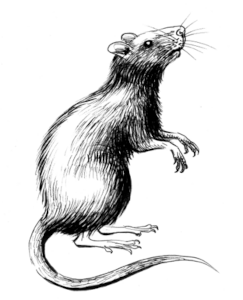
\includegraphics[scale=.2]{cunning/Rat}
\end{center}

  \mytable{l X}{
    \thead{d6} & \thead{Familiar}\\
  }{
    1 & The severed hands of a tomb robber  \\
    2 &  A floating piece of quartz \\
    3 & A 9-segmented colored cube that turns constantly  \\
    4 & A button-eyed doll made of rags and straw \\
    5 &  A tiny deformed homonculous resembling you \\
    6 & A hyper-intelligent slime \\
  }  



\OCCULT[
  Name=Damning,
  Link=occultism-damning,
  Pips=5,
  Time=Days
]

When you perform this ritual on a Mortal corpse no more than 7 days dead, you prevent them from departing \mylink{Limbo}{the-afterlife}.  The soul is trapped in Limbo permanently (though their soul can still be lead back to the Mortal plane through \mylink{Katabasis}{occultism-katabasis}).  The corpse is consumed when this ritual is performed.


\OCCULT[
  Name=Descry,
  Link=occultism-descry,
  Pips=See below,
  Time=Days
]

For each Cunning Pip you spend, you can see events transpiring 100km away (so 2 Pips, 200km; 3 Pips, 300km; etc.) by gazing into a silver bowl, censer, crystal ball, mirror, or other mystical item. This item must be a \mylink{Scrying Vessel}{marvels-scrying-vessel} (see \mylink{Marvels}{cunning-marvels} for more info).  You only need to describe what you want to see and it will appear, but the vision is misty and it's hard to make out details.  You can't see things that you might not normally be able to see, so if you said you wanted to "see the body of Sir Tremalane on the northern battlefield", and the body was buried, you might only see a grave.

The scrying doesn't have to only show events of the present; for each Cunning Pip you spend (apart from the Cunning Pips for seeing over great distances), you can see 1 century into the past. You'd have to have a rough idea of what you'd want to see - "show me the temples of Syrinx before they were cast down" would work, but "show me the secret entrance to the Caverns of Chaos" wouldn't.  The more detailed the description of what you want to see, the better you see it.

\example {
    Katarina wishes to see the location of a temple as it stood 200 years in the past, located somewhere in the jungle in the 100km surrounding the city. She must spend 3 Cunning Pips (2 for the years, 1 for the distance) to descry the location.
}

  \myimage{cunning/Occult_2}

\cbreak


\OCCULT[
  Name=Geas,
  Link=occultism-geas,
  Pips=10,
  Time=Days
]

A Geas is a command that compels the victim to perform a certain action, or fulfill a certain condition. The Geas could be long or difficult, like "find me the Needle of Obscurity in the Endless Haystacks" - or something easy, like "don't ever talk to me again." The victim must win a \RBTRY{\FOC}{\FOC} contest against you; if they fail, the Geas takes effect. From then on, any day that is not spent fulfilling the Geas will have one of the following effects (roll each day):


\callout {
\mynumlist {
  \item Inflicted with a \mylink{Greater Curse}{cunning-curses} (re-roll any duplicates);
  \item Inflicted with a \mylink{Disease}{vulgate-medicine-diseases} (roll on the Diseases table, re-roll any duplicates);
  \item Inflicted with a \mylink{Wound}{physical-wound} (roll on the Wounds table as if the target had been brought to 0 Flesh);
  \item All facets of \mylink{Personality}{adventurer-personality} move \DCDOWN;
  \item Inability to "heal" in any way - you gain absolutely no benefits from resting;
  \item Roll again - the result of the roll is inflicted on the target's loved one / parent / child / friend / etc. instead.  If the target loves nothing, the Arbiter gets to choose.
}
}

The effect lasts until sundown; provided the subject of the Geas is "back on track", the effect ends - otherwise, roll again.

The Geas must be doable, even if it is way above the means and possibility of the victim.  Should it become impossible (if the Endless Haystacks catch fire, for example), then the Geas is lifted.  Should you or the victim die, the Geas remains in effect, even if you are brought back from Limbo. This occultism cannot be performed on someone more than once in their lifetime.

On the upside, the Geas can empower its subject (at the Arbiter's discretion) to help them complete their task.  For example, if the Endless Haystacks are located in the fields outside of the cloud castle of the Giant King, the victim of the Geas might discover they have a handful of magic beans in their pocket that can help get them there.

The target of the Geas needs to be conscious and near you when you invoke the ritual.


\OCCULT[
  Name=Haunt,
  Link=occultism-haunt,
  Pips=5,
  Time=Days
]

You summon poltergeists to haunt an area up to 10km away. The area haunted has to be a distinct place (a graveyard, a house, etc.) no more than 100 square meters in size, and the haunting must be centered on a personal \mylink{Witch Mark}{occultism-witch-mark}. The poltergeists will cause chaos and mischief to any Mortals other than the invoker who enter their domain. They can neither talk nor directly harm anyone, but they will laugh unnervingly, appear as visible apparations, shake chains, throw things telekinetically about the room, etc. Meaningful rest (except a Breather) in a Haunted place is impossible, as is any ability or Arcana that requires Concentration. The grounds of the Haunting are considered \mylink{Unhallowed Earth}{occultism-unhallowed-earth}. The Haunting can only be ended by the removal of the Witch Mark (see description for methods of erasure).

\begin{center}
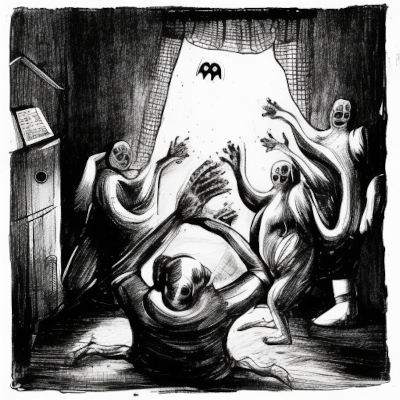
\includegraphics[scale=.45]{cunning/Poltergeist}
\end{center} 

\cbreak

  \myimage{cunning/Occult_3}

\OCCULT[
  Name=Hekaphage,
  Link=occultism-hekaphage,
  Pips=1+,
  Time=Days
]

\callout {
    For a Curse removed by a \mylink{Mundunugu}{gear-services}, multiply the costs by 5x (so 100\AG for a Lesser Curse and 500\AG for a Greater Curse).
}


You can destroy a curse by feeding it to a \mybold{Hekaphage}, an ethereal creature that eats Curses.  The number of pips required depends on the strength of the Curse:

\mybullet{
    \item a Lesser Curse requires 1 Cunning Pip
    \item a Greater Curse requires 5 Cunning Pips
}



\newpage


\OCCULT[
  Name=Katabasis,
  Link=occultism-katabasis,
  Pips=20,
  Time=Days
]

\summary {
    See the section on \mylink{the Afterlife}{the-afterlife} for more info about Limbo.
}

You open the door to \mylink{Limbo}{the-afterlife}, where the souls of the Hallowed dead must reside for 7 days before they rejoin the side of \TheAuthority. Mortals who pass through this door can attempt to bring a soul back to the land of the living.

The ritual must take place on \mylink{Unhallowed Earth}{occultism-unhallowed-earth}, in a room with a single door and no windows. By inhaling a special incense / partaking of a sacred mushroom / drinking a poisonous concoction / etc. up to 6 Mortals may pass through the door and enter the sorrowful plane of Limbo. The ritualist (you) must remain behind to keep the door open. You can keep the door open for as long as you \mylink{Concentrate}{time-concentration}; if your Concentration is broken, the door shuts, and those on the other side are lost.

Each Mortal who enters Limbo must carry a possession of the deceased: a sword, comb, lock of hair, etc. As long as they have this object in their possession, they have a rough idea of where the soul of the departed currently is. Additionally, they must bring two gold coins with them to pay the ferryman / conductor / guide / mayor / etc. who transports souls through Limbo, or use the coins to bribe ravens / make phonecalls / drop into wishing wells / etc.  The purpose of the coins seems to always vary, but anyone who walks through the door without these coins never returns. Finally, the Adventurers must carry a \mylink{Magic Jar}{marvels-magic-jar} (see \mylink{Marvels}{cunning-marvels}) through the doorway to transport the soul back home. A Magic Jar in Limbo attracts much attention ...

Once the soul is found, it must be placed into the Magic Jar to be transported across the threshold of Limbo. Manifold are the wonders of Limbo, and the soul may wish to remain rather than return to its humdrum life. It is better if a soul is coaxed within, rather than coerced. A Mortal can force a soul in Limbo into a Magic Jar against its will, but doing so consigns the vessel of the soul to permanent \mylink{Melancholy}{injury-insanity-madness}.

If a soul is successfully returned to the lands of the living, and their corpse is within the confines of the room, they may inhabit the body at no penalty (though an \INSANITY try is required).  If the corpse is absent, the Mortal will be reincarnated - the Player must move their Adventurer's Glory to the lowest number for their level (so if they were Level 7, they would move down to 32,000 Glory) and reroll their Adventurer.

Limbo will only permit a soul to be returned once. If a person should perish again, their souls become one of the \mylink{Forgotten}{the-forgotten}. Any Mortals that perish in Limbo are consumed in the same way.


\OCCULT[
  Name=Lichdom,
  Link=occultism-lichdom,
  Pips=20,
  Time=Months
]

This dangerous and depraved rite binds a Mortal's soul to a phylactery, allowing them to live on as a lich with life everlasting. Instead of the typical costs to perform a ritual, you must spend at least 25,000 \AU (higher costs at the Arbiter's discretion) for the necessary complex magical and chemical apparatus; bribes and dark gifts to creatures unholy creatures; hard-to-come-by components; etc. In addition to this exhorbitant sum, this rite requires:

\mybullet {
    \item a \mylink{Magic Jar}{marvels-magic-jar} (see \mylink{Marvels}{cunning-marvels}), which will become the Lich's phylactery;
    \item a dagger or knife marked with a \mybold{Bloodletting} rune (see \mylink{Sword Magic}{wonder-sword-magic}); and
    \item a Mortal vessel - that is, a human corpse - dead for less than 7 days
}

The ritual must take place in a room suitable for \mylink{Katabasis}{occultism-katabasis}. There, the deathly aspirant places their soul into the Magic Jar, stands in the doorway of Limbo, allows their jugular to be slit with the Bloodletting knife, and crosses the threshold with the Jar just as they expire.

\newpage

\myimage{cunning/Lichdom}

\cbreak

The Lich-to-be must bargain with the demons and devils of Limbo for life everlasting; their price should be high, and suitably depraved. Should the payment prove suitable, the Lich is permitted to return to the lands of the living carrying the Magic Jar with their soul inside.

The Magic Jar of this unholy creature is known as a \mybold{Phylactery}; so long as it remains intact, the Lich will live forever. If a Lich is slain, it will reform near their Phylactery at the next sunset. Liches have all of the powers, abilities, and memories they had in their Mortal form, and an endless amount of time to learn new things. In addition:

\callout{
\mybullet {
    \item The Lich ages one year for every 10 years that pass (very old liches tend to look cadaverous or skeletal);
    \item The Lich is immune to non-magical weapons, \mylink{Toxins}{malignants-toxins}, \mylink{Secrets of the Mind}{arcana-wizardry-secrets-alignment}, and \mylink{Secrets of Entropy}{arcana-wizardry-secrets-alignment}; and
    \item If the Lich knows any Secrets, they may write as many of them as they desire into their skulls (see \mylink{Sorcerer's Skull}{arcana-wizardry-skull} under \mylink{Wizardry}{arcana-wizardry}) - making them extremely potent Fetishes in their own right!
}}

Liches are \mybold{Unhallowed}. If their phylactery is destroyed or opened, they immediately disappear in a dazzling flash, their souls returned to Limbo for eternal torment. 

\newpage

\OCCULT[
  Name=Malison,
  Link=occultism-malison,
  Pips=2+,
  Time=Days
]

You place a \mylink{Curse}{cunning-curses} ...

\mylist {
  \item ... on a person within 1km; 
  \item ... on a \mylink{Marvel}{cunning-marvels};  
  \item ... on your \mylink{Familiar}{occultism-familiars}; or
  \item ... on a \mylink{Cursing Sigil}{inscription-sigil-cursing}
}

The cost varies:

\mybullet{
    \item a \myital{random} Lesser Curse requires 2 Cunning Pips.
    \item a \myital{specific} Lesser Curse requires 6 Cunning Pips.
    \item a \myital{random} Greater Curse requires 10 Cunning Pips.
    \item a \myital{specific} Greater Curse requires 14 Cunning Pips.

}

You can break any of your own curses at will. Malisons will survive your death.  \mylink{Pooka}{species-pooka} are immune to your Malison.

\cbreak

\OCCULT[
  Name=Unhallowed Earth,
  Link=occultism-unhallowed-earth,
  Pips=2,
  Time=Days
]

Through the Occultism of Unhallowed Earth, you desecrate a handful of earth and imbue it with the chaos energy of the Void. Unhallowed Earth must be stored in a \mylink{Witch Bottle}{marvels-witch-bottle} until you are ready to use it. When poured on the ground, the soil desecrates an area 10 meters in radius. If the ground that is desecreated is \mylink{Hallowed Ground}{miracle-hallowed-ground}, the blessing is removed. Otherwise no Mortal or Hallowed creature may enter Unhallowed Earth unless they are invited by the Mystic who created it or they bear their \mylink{Witch Mark}{occultism-witch-mark}; and no \mylink{Sacraments}{vulgate-sacraments} may be performed on its soil.



\OCCULT[
  Name=Witch Mark,
  Link=occultism-witch-mark,
  Pips=1,
  Time=Days
]

A smear of the Void is placed on a person or thing, only visible to the Unseelie and to Mortals using the Charm of the \mylink{Third Eye}{vulgate-charms} (see the \mylink{Vulgate of Charms}{vulgate-charms}). Your Witch Mark is unique, like a fingerprint or calling card. Unless you've seen a particular Witch Mark before, a \mylink{Skill: Lore}{skill-lore} try is required to determine the owner of the Witch Mark. Mortal creatures marked with a Witch Mark are \mybold{Unhallowed} for either 7 days or until the end of the Session (whichever comes first); otherwise, a Witch Mark can only be removed by the witch who placed it there, or by sprinkling the symbol with a pinch of \mylink{Hallowed Ground}{miracle-hallowed-ground}.
